\subsection{Einzelnes Gerät}
In diesem Abschnitt werden die Ergebnise erwähnt, welche durch ein einzelnes Gerät entstehen. Jedes dieser Geräte speichert die gesammelten Daten in einem Feature Vektor ab. Die folgende Abbildung (\fref{bFVec}) zeigt zehn Einträge eines solchen Feature Vektors.

\begin{figure}[H]
  \centering
  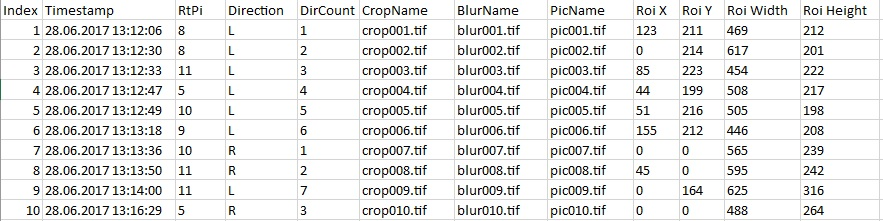
\includegraphics[width=1\textwidth]{Resultate/FeatureVector.jpg} 
  \caption{Feature Vektor eines einzelnen Gerätes.}
  \label{bFVec}
\end{figure}

\subsubsection{Zählen}
Durch den Einsatz eines einzelnen Gerätes kann an den Aufstellpunkten die Anzahl der vorbeifahrenden Verkehrsteilnehmer gezählt werden. An jedem dieser Punkte erhält der Bediener die Anzahl der Verkehrsteilnehmer, welche in das Gebiet hinein- und welche  aus dem Gebiet heraus fahren. Ebenso enthält jedes dieser gezählten Verkehrsteilnehmer  eine fortlaufende Nummer, einen Zeitstempel und die Information über dessen Fahrtrichtung.

\subsubsection{Kategorisieren}
Jedes Einzelgerät ist ebenso im Stande die vorbeifahrenden Verkehrsteilnehmer in vordefinierte Kategorien einzuteilen. Dabei wird die Anzahl an Pixeln, welche sich bewegen, gezählt. Dadurch kann eine quantitative Kategorisierung in drei Kategorien geschehen. Wie in \fref{bNachverarbeitung} in Spalte drei zu sehen ist, werden die Kategorien in "'NV"', "'1"' und "'2"' eingeteilt. "'NV"' sind Verkehrsteilnehmer, welche kleiner als ein Auto sind. Die "'1"' gibt an, dass es sich um ein Auto handelt. Die Nummer "'2"' deutet darauf hin, dass es sich um grössere Verkehrsteilnehmer handelt.

\subsubsection{Geschwindigkeitserkennung}
Die Geschwindigkeit der Verkehrsteilnehmer dient als Indikator, wie schnell tatsächlich an den Geräten vorbei gefahren wird. Ein Grossteil der Fahrzeuglenker reduzieren ihre Geschwindigkeit, falls sie merken, dass diese aufgezeichnet wird. Da sich "'Fast and Curious"' auf einer Höhe von sechs Metern befindet, werden diese Geräte von den meisten Verkehrsteilnehmern nicht erkannt, weshalb diese ohne die Geschwindigkeit zu Drosseln vorbei fahren. Aufgrund dessen kann die tatsächliche Geschwindigkeit besser errechnet werden.\\\\
Die Geschwindigkeit kann aus zwei aufeinanderfolgenden Frames extrahiert werden. Dabei wird der Positionsunterschied der Fahrzeuge auf den Frames verwendet. Um die Geschwindigkeit berechnen zu können, wurde eine Referenzmessung durchgeführt, bei welcher zwischen zwei aufeinanderfolgenden Frames, eine Verschiebung von 58 Pixeln pro km/h gemessen wurde. Nun konnte durch eine einfache Schlussrechnung die Geschwindigkeit der Verkehrsteilnehmer berechnet werden. Dabei wird der Positionsunterschied, in Pixeln, durch die Referenzmessung geteilt. Das Ergebnis dabei ist die Geschwindigkeit des Fahrzeugs. Bei größeren Fahrzeugen, wie einem LKW oder einem Traktor, wurde die Verschiebung von 58 Pixeln pro km/h auf 25 Pixeln pro km/h gesenkt, da die Kanten dieser Fahrzeuge näher an der Kamera sich befinden. Auf \fref{bNachverarbeitung} in Spalte sechs, sind die berechneten Geschwindigkeiten dargestellt. Mit einem frei wählbaren Farbcode wurde das Ergebnis markiert. Für eine besser Veranschaulichung wurde zudem ein Diagramm (\fref{bGeschwDiagramm}) hinzugefügt. Darauf ist ersichtlich, dass der grösste Teil der Verkehrsteilnehmer sich beinahe an die maximale Höchstgeschwindigkeit von  50 km/h  im Dorf hielt. Dennoch wurden auch Geschwindigkeiten weit über der maximal tollerierten Höchstgeschwindigkeit gemessen.

\begin{figure}[H]
  \centering
  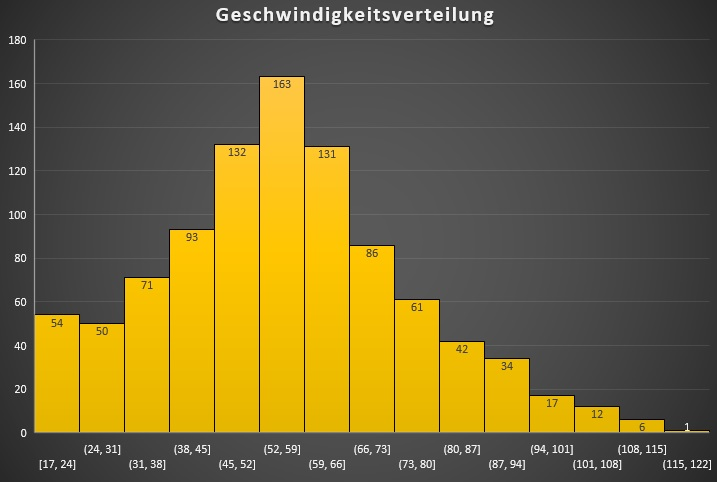
\includegraphics[width=0.6\textwidth]{Resultate/GeschwDiagramm.jpg} 
  \caption{Diagramm der Geschwindigkeitsverteilung auf einer 50er Strasse am Ende eines Dorfes.}
  \label{bGeschwDiagramm}
\end{figure}

\begin{figure}[H]
  \centering
  \subfigure[Geschwindigkeitsverteilung Auto und Motorrad]{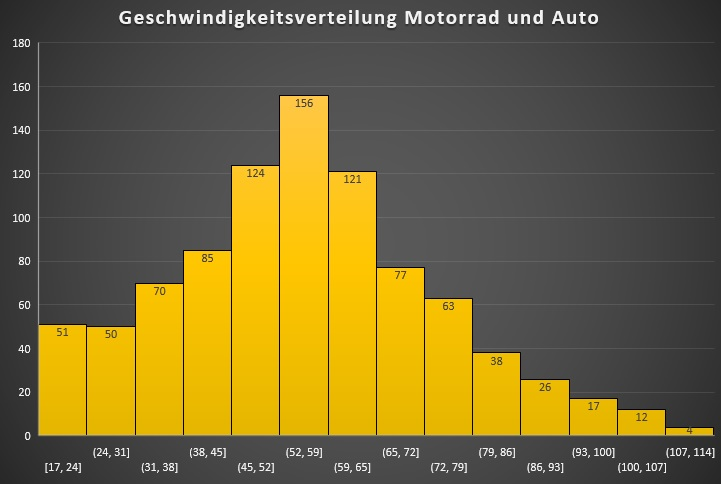
\includegraphics[width=0.47\textwidth]{Resultate/GeschwDiagrammAutoMotorrad.jpg}}
  \subfigure[Geschwindigkeitsverteilung grössere Fahrzeuge]{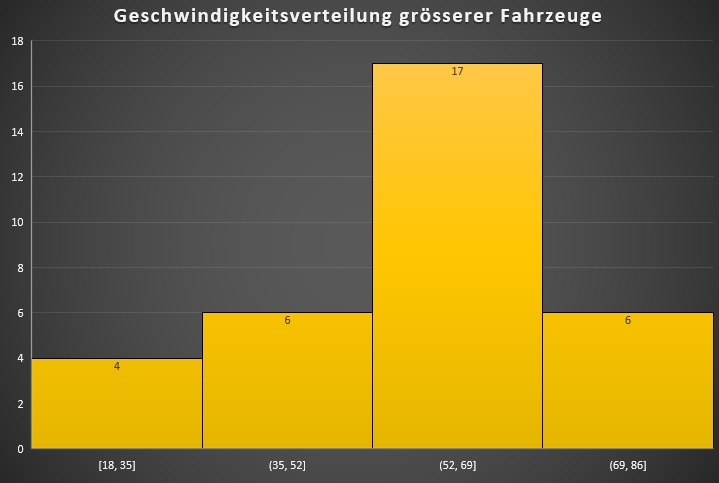
\includegraphics[width=0.47\textwidth]{Resultate/GeschwDiagrammLKW.jpg}}
  \caption{Geschwindigkeitsverteilung aufgetrennt in die Kategorien kleine und grosse Fahrzeuge.}
  \label{bFrames}
\end{figure}

\begin{figure}[H]
  \centering
  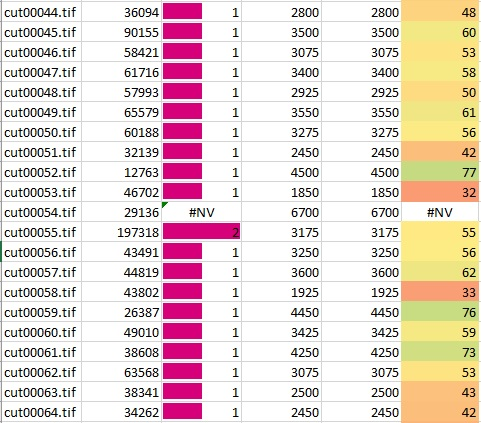
\includegraphics[width=0.58\textwidth]{Resultate/Nachverarbeitung.jpg} 
  \caption{Tabelle des nachverarbeiteten Feature Vektors.}
  \label{bNachverarbeitung}
\end{figure}